\documentclass[11pt, a4paper]{article}

% ==========================================
% --- UNIVERSAL PREAMBLE (modèle ENSET) ---
% ==========================================
\usepackage[a4paper, top=2.5cm, bottom=2.5cm, left=2.5cm, right=2.5cm]{geometry}
\usepackage{fontspec}
\usepackage[french]{babel}
\setmainfont{Noto Serif}
\setsansfont{Noto Sans}
\setmonofont{Noto Sans Mono}

\usepackage{graphicx}
\usepackage{grffile}
\graphicspath{{../screens/}{images/}{uml/}}
\usepackage{float}
\usepackage{xcolor}
\usepackage{colortbl}
\usepackage{listings}
\usepackage{caption}
\usepackage{fancyhdr}
\usepackage{titlesec}
\usepackage[most]{tcolorbox}
\usepackage{booktabs}
\usepackage{tabularx}
\usepackage{tikz}
\usetikzlibrary{positioning, arrows.meta, calc, shapes.geometric}
\usepackage{amsmath}
\usepackage{amssymb}
\usepackage{enumitem}
\usepackage{tocloft}
\usepackage{hyperref}
\usepackage{xurl}
\urlstyle{same}

% Retour à la ligne optimal en français (XeLaTeX uniquement)
\ifdefined\XeTeXlinebreaklocale
  \XeTeXlinebreaklocale "fr"
  \XeTeXlinebreakskip = 0pt plus 1pt
\fi
\emergencystretch=2.5em
\setlength{\hfuzz}{3pt}
\newcommand{\longpath}[1]{\texttt{\footnotesize\hyphenchar\font=`\-\relax #1}}
\lstdefinestyle{jsonout}{
  basicstyle=\small\ttfamily,
  breaklines=true,
  breakatwhitespace=false,
  columns=fullflexible,
  keepspaces=true,
  showstringspaces=false,
  frame=none,
  aboveskip=4pt,
  belowskip=4pt,
}

% --- Variables du document ---
\newcommand{\ecole}{ENSET MOHAMMEDIA}
\newcommand{\filiere}{Master SDIA --- SMA}
\newcommand{\annee}{Année Universitaire 2025--2026}
\newcommand{\module}{Systèmes Distribués et Intelligence Artificielle --- Technologies Web}
\newcommand{\typedoc}{Rapport de Projet}
\newcommand{\sujet}{Mourchid : Assistant académique ENSET\\[0.2em]multi-agent avec RAG agentique}
\newcommand{\equipe}{%
  Ahmed DOUYRY\\[0.15cm]Yazid ESSOKTANI\\[0.15cm]Imane MEKKAOUI%
}
\newcommand{\encadrant}{Oumaima AGHERAI}
\newcommand{\dateRendu}{Juin 2026}
\newcommand{\repoGit}{https://github.com/ahmed-douyry/enset-assistant}

% --- Couleurs ---
\definecolor{mypurple}{HTML}{6B21A8}
\definecolor{mypurplelight}{HTML}{F3E8FF}
\definecolor{myred}{HTML}{E11D48}
\definecolor{darkbg}{HTML}{1E1E1E}
\definecolor{codegray}{HTML}{F8F9FA}
\definecolor{lightbg}{HTML}{F8FAFC}
\definecolor{darkblue}{HTML}{1E293B}
\definecolor{ubuntubg}{HTML}{300A24}
\definecolor{ubuntubar}{HTML}{1E1E1E}
\definecolor{ubuntutext}{HTML}{EEEEEC}
\definecolor{ubuntugreen}{HTML}{8AE234}
\definecolor{ubuntucyan}{HTML}{34E2E2}
\definecolor{draculabg}{HTML}{000000}
\definecolor{draculafg}{HTML}{F8F8F2}
\definecolor{draculacomment}{HTML}{6272A4}
\definecolor{draculapink}{HTML}{FF79C6}
\definecolor{draculayellow}{HTML}{F1FA8C}
\definecolor{draculacyan}{HTML}{8BE9FD}
\definecolor{draculaorange}{HTML}{FFB86C}
\definecolor{draculagreen}{HTML}{50FA7B}
\definecolor{macred}{HTML}{FF5F56}
\definecolor{macyellow}{HTML}{FFBD2E}
\definecolor{macgreen}{HTML}{27C93F}
\definecolor{warnbg}{HTML}{FFFBEB}
\definecolor{warnframe}{HTML}{B45309}
\definecolor{warnaccent}{HTML}{F59E0B}
\definecolor{infobg}{HTML}{EFF6FF}
\definecolor{infoframe}{HTML}{1D4ED8}
\definecolor{infoaccent}{HTML}{3B82F6}
\definecolor{successbg}{HTML}{ECFDF5}
\definecolor{successframe}{HTML}{047857}
\definecolor{videobg}{HTML}{F5F3FF}

\hypersetup{colorlinks=true, linkcolor=mypurple, urlcolor=mypurple, citecolor=myred}
\tcbuselibrary{listings}

\setlist[itemize,1]{label=\textcolor{mypurple}{\textbullet}, leftmargin=*}
\setlist[itemize,2]{label=\textcolor{mypurple!60}{\circ}, leftmargin=*}

\pagestyle{fancy}
\fancyhf{}
\setlength{\headheight}{22pt}
\fancyhead[L]{\fontsize{9}{11}\sffamily\color{gray} \module}
\fancyhead[R]{\fontsize{9}{11}\sffamily\color{gray} \filiere}
\fancyfoot[C]{\sffamily\thepage}
\renewcommand{\headrulewidth}{0.4pt}
\renewcommand{\headrule}{\hbox to\headwidth{\color{mypurple!30}\leaders\hrule height \headrulewidth\hfill}}

\renewcommand{\cftsecfont}{\sffamily\bfseries\color{mypurple}}
\renewcommand{\cftsecpagefont}{\sffamily\color{gray}}
\renewcommand{\cftsecleader}{\cftdotfill{\cftsecdotsep}}
\renewcommand{\cftsecdotsep}{\cftdot}
\setlength{\cftsecindent}{0pt}
\setlength{\cftsecnumwidth}{2em}
\renewcommand{\cftsubsecfont}{\sffamily\color{gray!80!black}}
\renewcommand{\cftsubsecpagefont}{\sffamily\color{gray}}
\renewcommand{\cftsubsecleader}{\cftdotfill{\cftsubsecdotsep}}
\renewcommand{\cftsubsecdotsep}{\cftdot}
\setlength{\cftsubsecindent}{2em}
\setlength{\cftsubsecnumwidth}{2.5em}
\setlength{\cftbeforesecskip}{5pt}
\setlength{\cftbeforesubsecskip}{2pt}

\titleformat{\section}{\normalfont\Large\bfseries\sffamily\color{mypurple}}{\thesection.}{0.5em}{}[\vspace{0.2ex}\color{mypurple!20}\titlerule]
\titleformat{\subsection}{\normalfont\large\bfseries\sffamily\color{gray!80!black}}{\thesubsection}{1em}{}

\lstdefinestyle{draculastyle}{
    language=Python,
    backgroundcolor=\color{draculabg},
    basicstyle=\ttfamily\footnotesize\color{draculafg},
    keywordstyle=\color{draculapink}\bfseries,
    stringstyle=\color{draculayellow},
    commentstyle=\color{draculacomment}\itshape,
    numbers=left,
    numberstyle=\tiny\color{draculacomment},
    numbersep=14pt,
    xleftmargin=22pt,
    breaklines=true,
    tabsize=4,
    emph={def, return, class, from, import, as, pass, if, elif, else, for, while, in, async, await},
    emphstyle=\color{draculapink}\bfseries,
    emph={[2]StateGraph, TypedDict, add_node, add_edge, add_conditional_edges},
    emphstyle={[2]\color{draculaorange}},
    emph={[3]LegalGraphState, graph, ainvoke},
    emphstyle={[3]\color{draculacyan}}
}

\newcommand{\greencheck}{%
  \begin{tikzpicture}[baseline=-0.3em]
    \draw[macgreen, line width=1.5pt, line cap=round, line join=round] (0,0.15) -- (0.15,0) -- (0.4,0.4);
  \end{tikzpicture}%
}
\newcommand{\redcross}{%
  \begin{tikzpicture}[baseline=-0.3em]
    \draw[myred, line width=1.5pt, line cap=round] (0,0) -- (0.3,0.3) (0,0.3) -- (0.3,0);
  \end{tikzpicture}%
}
\newcommand{\warnicon}{%
  \begin{tikzpicture}[baseline=-0.35em, scale=0.9]
    \fill[warnaccent] (0,0.35) -- (-0.42,-0.32) -- (0.42,-0.32) -- cycle;
    \node[font=\sffamily\bfseries\scriptsize, text=warnbg] at (0,0) {!};
  \end{tikzpicture}%
}
\newcommand{\infoicon}{%
  \begin{tikzpicture}[baseline=-0.3em]
    \fill[infoaccent] (0,0) circle (0.45em);
    \node[text=white, font=\sffamily\bfseries\tiny] at (0,0) {i};
  \end{tikzpicture}%
}
\newcommand{\webicon}{%
  \begin{tikzpicture}[baseline=-0.3em, scale=0.8]
    \draw[mypurple, thick] (0,0) circle (0.6em);
    \draw[mypurple, thick] (0,-0.6em) .. controls (0.3em,-0.3em) and (0.3em,0.3em) .. (0,0.6em);
    \draw[mypurple, thick] (-0.6em,0) -- (0.6em,0);
  \end{tikzpicture}%
}

\newtcolorbox{focusbox}[1][Focus]{
  enhanced, breakable, colback=mypurplelight!55, colframe=mypurple, boxrule=1pt, arc=6pt,
  drop fuzzy shadow=gray!25,
  title={\sffamily\bfseries #1}, coltitle=white,
  attach boxed title to top left={xshift=15pt, yshift=-10pt},
  boxed title style={colback=mypurple, arc=3pt, boxrule=0pt},
  top=15pt, bottom=10pt, left=15pt, right=15pt
}
\newtcolorbox{citationbox}{
  enhanced, breakable, frame hidden, colback=mypurplelight!40,
  borderline west={4pt}{0pt}{mypurple}, fontupper=\itshape\color{darkblue},
  before skip=1.5em, after skip=1.5em, top=12pt, bottom=12pt, left=14pt, right=12pt
}
\newtcolorbox{alertwarning}[1][Attention]{
  enhanced, breakable, colback=warnbg, colframe=warnframe!40, boxrule=0pt, arc=6pt,
  borderline west={4pt}{0pt}{warnaccent},
  title={\warnicon\quad\sffamily\bfseries\textcolor{warnframe}{#1}},
  fonttitle=\sffamily, attach title to upper,
  after title={\par\vspace{0.25em}},
  top=10pt, bottom=10pt, left=12pt, right=12pt
}
\newtcolorbox{alertinfo}[1][Information]{
  enhanced, breakable, colback=infobg, colframe=infoframe!35, boxrule=0pt, arc=6pt,
  borderline west={4pt}{0pt}{infoaccent},
  title={\infoicon\quad\sffamily\bfseries\textcolor{infoframe}{#1}},
  fonttitle=\sffamily, attach title to upper,
  after title={\par\vspace{0.25em}},
  top=10pt, bottom=10pt, left=12pt, right=12pt
}
\newtcolorbox{alertsuccess}[1][Succès]{
  enhanced, breakable, colback=successbg, colframe=successframe!35, boxrule=0pt, arc=6pt,
  borderline west={4pt}{0pt}{successframe},
  title={\greencheck\quad\sffamily\bfseries\textcolor{successframe}{#1}},
  fonttitle=\sffamily, attach title to upper,
  after title={\par\vspace{0.25em}},
  top=10pt, bottom=10pt, left=12pt, right=12pt
}
\newcounter{stepcounter}
\newtcolorbox{etapebox}[1][]{
  enhanced, colback=infobg!50, colframe=infoaccent!50, boxrule=0.6pt, arc=6pt,
  left=35pt, right=10pt, top=10pt, bottom=10pt,
  drop fuzzy shadow=gray!12, before={\stepcounter{stepcounter}},
  overlay={
    \node[fill=infoaccent, text=white, circle, inner sep=0pt, minimum size=20pt, font=\sffamily\bfseries]
      at ([xshift=22pt]frame.west) {\thestepcounter};
  }, #1
}
\newenvironment{infobox}[1][Remarque]{\begin{alertinfo}[#1]}{\end{alertinfo}}
\newtcblisting{terminalbox}[1][]{
  enhanced,
  colback=ubuntubg,
  colframe=ubuntubar,
  colbacktitle=ubuntubar,
  arc=5pt,
  boxrule=1pt,
  drop fuzzy shadow=gray!30,
  fonttitle=\sffamily,
  coltitle=white,
  top=0pt,
  bottom=0pt,
  left=2pt,
  right=5pt,
  title={
     \makebox[0pt][l]{\textcolor{gray!60}{\scriptsize\sffamily >\_}}%
     \hfill\textcolor{white!90}{\scriptsize\sffamily #1}\hfill
     \makebox[0pt][r]{%
       \tikz{\fill[gray!40] (0,0) circle (3.5pt); \draw[darkgray, line width=0.5pt] (-1.5pt,0) -- (1.5pt,0);}~%
       \tikz{\fill[gray!40] (0,0) circle (3.5pt); \draw[darkgray, line width=0.5pt] (-1.5pt,-1.5pt) rectangle (1.5pt,1.5pt);}~%
       \tikz{\fill[gray!40] (0,0) circle (3.5pt); \draw[darkgray, line width=0.5pt] (-1.5pt,-1.5pt) -- (1.5pt,1.5pt) (-1.5pt,1.5pt) -- (1.5pt,-1.5pt);}%
     }
  },
  listing only,
  listing options={
      xleftmargin=0pt,
      xrightmargin=0pt,
      language={},
      basicstyle=\ttfamily\footnotesize\color{ubuntutext},
      identifierstyle=\color{ubuntutext},
      keywordstyle=\color{ubuntutext},
      stringstyle=\color{ubuntutext},
      backgroundcolor=\color{ubuntubg},
      numbers=none,
      breaklines=true,
      escapeinside={(*@}{@*)},
      showstringspaces=false,
      columns=fullflexible,
      keepspaces=true
  }
}
\newtcblisting{vscodebox}[2][]{
  enhanced,
  colback=draculabg,
  colframe=gray!15!black,
  arc=6pt,
  boxrule=1pt,
  drop fuzzy shadow=gray!40,
  fonttitle=\sffamily,
  coltitle=white,
  top=0pt,
  bottom=0pt,
  left=0pt,
  right=5pt,
  title={
    \vspace{2pt}
    \makebox[\linewidth]{%
    \hspace{4pt}
      \begin{tikzpicture}[baseline=-0.3em]
        \fill[macred] (0,0) circle (3pt);
        \fill[macyellow] (0.45,0) circle (3pt);
        \fill[macgreen] (0.9,0) circle (3pt);
      \end{tikzpicture}%
      \hfill
      \textcolor{draculacyan}{\textbf{\{\ \}}}\ %
      \textcolor{draculafg!80}{\footnotesize\sffamily\bfseries #2}
      \hfill
      \hspace{1.2cm}
    }%
  },
  listing only,
  listing options={style=draculastyle, #1}
}

\newcommand{\ftdir}[1]{\textcolor{mypurple}{\sffamily\bfseries $\blacktriangleright$}\ \textbf{#1}\par\vspace{0.15em}}
\newcommand{\ftitem}[2]{\hspace{1.4em}\textcolor{draculacyan}{\texttt{$\circ$}}\ \texttt{#1}\hfill{\footnotesize\sffamily\color{gray!65}#2}\par\vspace{0.1em}}
\newenvironment{filetree}{%
  \begin{tcolorbox}[enhanced, colback=codegray, colframe=mypurple!35, arc=6pt, boxrule=0.8pt,
    left=10pt, right=10pt, top=10pt, bottom=10pt,
    fontupper=\ttfamily\footnotesize, drop fuzzy shadow=gray!20]
}{%
  \end{tcolorbox}%
}

% Commande UML : titre coloré + liste d'attributs
% #2 n'est PAS entouré de {} : \\ peut agir comme saut de ligne de tableau
\newcommand{\umlbox}[2]{%
  \setlength{\arrayrulewidth}{0.4pt}%
  \begin{tabular}{|>{\ttfamily\scriptsize}l|}
    \hline
    \cellcolor{mypurple}\textcolor{white}{\sffamily\bfseries\scriptsize #1}\\
    \hline
    #2\\
    \hline
  \end{tabular}%
}

\newcommand{\screenshot}[3]{%
  \begin{figure}[H]
    \centering
    \includegraphics[width=#1\textwidth]{#2}
    \caption{#3}
    \label{fig:#2}
  \end{figure}%
}

% ==========================================
\begin{document}

% --- PAGE DE GARDE ---
\begin{titlepage}
\begin{tikzpicture}[remember picture, overlay]
    \fill[lightbg] (current page.south west) rectangle (current page.north east);
    \fill[darkblue] (current page.north west) -- (current page.north east) -- ([yshift=-6cm]current page.north east) -- ([yshift=-3cm]current page.north west) -- cycle;
    \fill[mypurple] (current page.north east) -- ++(-10,0) -- ++(10,-7) -- cycle;
    \fill[myred] (current page.north east) -- ++(-4,0) -- ++(4,-3) -- cycle;
    \foreach \x in {0,0.5,...,10}
        \foreach \y in {0,0.5,...,5}
            \fill[white!20] ([xshift=\x cm, yshift=-\y cm-1cm]current page.north west) circle (1pt);
\end{tikzpicture}

\vspace*{-1cm}
\begin{minipage}[t]{0.5\textwidth}
    \begin{tcolorbox}[colback=white, colframe=white, boxrule=0pt, arc=5pt, width=5cm, height=2cm, valign=center, halign=center, shadow={2pt}{-2pt}{0pt}{black!10}]
        
\includegraphics[width=4cm, height=1.5cm, keepaspectratio]{images/logo_enset.png}
    \end{tcolorbox}
\end{minipage}
\hfill
\begin{minipage}[t]{0.45\textwidth}
    \vspace*{-1cm}
    \raggedleft
    \textcolor{white}{\sffamily\bfseries\Large \ecole}\\[0.2cm]
    \textcolor{white!90}{\sffamily\large \filiere}\\[0.1cm]
    \textcolor{white!80}{\sffamily\small \annee}
\end{minipage}

\vspace*{5cm}

\begin{center}
    \begin{tcolorbox}[
        enhanced,
        colback=white,
        colframe=mypurple,
        arc=15pt,
        boxrule=0pt,
        leftrule=10pt,
        drop large lifted shadow=black!20,
        top=1.5cm, bottom=1.5cm, left=1cm, right=1cm
    ]
        \centering
        {\textcolor{gray}{\sffamily\Large \module} \par}
        \vspace*{0.8cm}
        {\textcolor{darkblue}{\fontsize{32}{38}\selectfont\sffamily\bfseries \typedoc} \par}
        \vspace*{0.6cm}
        \begin{tikzpicture}
            \draw[myred, line width=2pt] (0,0) -- (3,0);
        \end{tikzpicture}
        \vspace*{0.6cm}
        {\textcolor{mypurple}{\LARGE\sffamily\bfseries \sujet} \par}
    \end{tcolorbox}
\end{center}

\vfill

\begin{minipage}[b]{0.48\textwidth}
    \begin{tcolorbox}[enhanced, colback=darkblue, colframe=darkblue, arc=8pt, fontupper=\color{white}, top=15pt, bottom=15pt]
        \sffamily\small RÉALISÉ PAR :\\[0.2cm]
        {\normalsize\bfseries \equipe}\\[0.4cm]
        \webicon\ \href{\repoGit}{\textcolor{white!80}{\footnotesize github.com/ahmed-douyry/enset-assistant}}
    \end{tcolorbox}
\end{minipage}
\hfill
\begin{minipage}[b]{0.48\textwidth}
    \begin{tcolorbox}[enhanced, colback=white, colframe=gray!20, arc=8pt, top=15pt, bottom=15pt]
        \raggedleft
        \sffamily\small ENCADRÉ PAR :\\[0.2cm]
        {\large\bfseries\textcolor{darkblue}{\encadrant}}\\[0.4cm]
        \textcolor{gray}{\footnotesize Fait le: \dateRendu}
    \end{tcolorbox}
\end{minipage}

\vspace*{0.5cm}
\end{titlepage}

% --- TABLE DES MATIÈRES ---
\newpage
\pagestyle{empty}
\vspace*{1cm}
\begin{center}
  {\sffamily\bfseries\fontsize{24}{28}\selectfont\color{mypurple}TABLE DES MATIÈRES}
\end{center}
\vspace{1.2cm}
\begingroup
\sffamily
\renewcommand{\contentsname}{}
\setcounter{tocdepth}{2}
\tableofcontents
\endgroup
\newpage
\pagestyle{fancy}

% =============================================================================
\section{Introduction}

\begin{focusbox}[Contexte académique]
Ce projet est réalisé dans le cadre du module \textbf{Systèmes Distribués et Intelligence Artificielle --- Technologies Web} du \textbf{Master SDIA} à l'\textbf{ENSET Mohammedia} (Université Hassan II de Casablanca). Il vise à concevoir et implémenter une application web complète intégrant des composants d'intelligence artificielle distribués.
\end{focusbox}

\subsection{Présentation du projet}

\textbf{Mourchid} est un assistant académique intelligent et \textbf{local-first} dédié aux étudiants et futurs candidats de l'\textbf{ENSET Mohammedia}. Il permet de rechercher, comprendre et structurer des informations relatives à la vie académique de l'école : filières du cycle ingénieur, procédures d'inscription, bourses, stages/PFE, clubs étudiants et concours d'accès.

\begin{citationbox}
« Mourchid » (مرشد) signifie \textit{guide} en arabe — métaphore choisie pour exprimer la vocation de l'assistant : orienter l'étudiant dans ses démarches académiques à partir de sources documentaires vérifiées.
\end{citationbox}

\subsection{Objectifs du projet}

\begin{itemize}
    \item Fournir un \textbf{assistant conversationnel intelligent} capable de répondre aux questions académiques en se basant sur un corpus de documents officiels ENSET.
    \item Implémenter un \textbf{pipeline RAG agentique} (Retrieval-Augmented Generation) multi-agent orchestré par \textbf{LangGraph}.
    \item Intégrer des fonctionnalités innovantes : \textbf{dictée vocale} avec transcription locale (Whisper), \textbf{quiz concours} générés par l'IA, visualisation du workflow multi-agent.
    \item Assurer une architecture \textbf{100\% locale et open-source}, sans dépendance à des APIs cloud propriétaires.
    \item Respecter les bonnes pratiques \textbf{Technologies Web} : API REST, streaming SSE, interface React responsive.
\end{itemize}

\begin{alertwarning}[Avertissement]
Les documents fournis dans le corpus sont des \textbf{échantillons pédagogiques} à titre de démonstration. L'assistant ne remplace pas le service de scolarité de l'ENSET ni les communications officielles de l'UH2C. Pour toute décision administrative, se référer aux services compétents.
\end{alertwarning}

% =============================================================================
\section{Cahier des charges}

\subsection{Problématique}

Les étudiants souhaitant intégrer l'ENSET Mohammedia ou déjà inscrits font face à plusieurs difficultés récurrentes :

\begin{itemize}
    \item \textbf{Dispersion de l'information} : les renseignements sur les filières, les procédures administratives (inscription, bourse, attestations), les clubs et les emplois du temps sont éparpillés sur plusieurs supports.
    \item \textbf{Manque de disponibilité} : le service de scolarité n'est pas accessible en dehors des heures de bureau.
    \item \textbf{Préparation insuffisante au concours} : les candidats manquent d'outils interactifs pour s'entraîner aux QCM par filière.
    \item \textbf{Barrière de langue et de format} : les documents officiels sont souvent denses et difficiles à parcourir.
\end{itemize}

\subsection{Besoins identifiés}

\begin{table}[H]
    \centering
    \sffamily
    \renewcommand{\arraystretch}{1.4}
    \begin{tabularx}{\textwidth}{>{\bfseries}p{3.5cm} X}
        \toprule
        \rowcolor{mypurple}
        \textcolor{white}{Catégorie} & \textcolor{white}{Besoins} \\
        \midrule
        Fonctionnels & Répondre aux questions académiques en langage naturel, proposer des procédures étape par étape, générer des résumés de documents, entraîner aux quiz concours. \\
        \rowcolor{codegray}
        Accessibilité & Interface disponible 24h/24, saisie par clavier ou voix (dictée vocale). \\
        Transparence & Citer les sources utilisées, afficher le score de confiance, permettre l'audit du pipeline agent. \\
        \rowcolor{codegray}
        Performance & Réponses en streaming (pas d'attente bloquante), interface réactive. \\
        Souveraineté & Fonctionnement 100\% local, aucune donnée envoyée à des serveurs tiers. \\
        \bottomrule
    \end{tabularx}
    \caption{Synthèse des besoins identifiés.}
\end{table}

\subsection{Solutions proposées}

\begin{table}[H]
    \centering
    \sffamily
    \renewcommand{\arraystretch}{1.4}
    \begin{tabularx}{\textwidth}{>{\bfseries}p{3.8cm} X c}
        \toprule
        \rowcolor{mypurple}
        \textcolor{white}{Problème} & \textcolor{white}{Solution retenue} & \textcolor{white}{Statut} \\
        \midrule
        Information dispersée & Pipeline RAG (Qdrant + SentenceTransformers) sur un corpus ENSET unifié & \greencheck \\
        \rowcolor{codegray}
        Disponibilité & Application web accessible en permanence sur \texttt{localhost:5173} & \greencheck \\
        Saisie difficile & Bouton micro + transcription Whisper locale côté serveur + barre de fréquence & \greencheck \\
        \rowcolor{codegray}
        Préparation concours & Quiz QCM générés par le LLM à chaque essai (par filière, par difficulté) & \greencheck \\
        Réponses opaques & Score de confiance, citations RAG, panneau workflow, traces persistées & \greencheck \\
        \rowcolor{codegray}
        Dépendance cloud & Stack 100\% locale : Ollama, Qdrant, Whisper, SentenceTransformers & \greencheck \\
        \bottomrule
    \end{tabularx}
    \caption{Cartographie problèmes $\leftrightarrow$ solutions.}
\end{table}

% =============================================================================
\section{Conception fonctionnelle}

\subsection{Identification des acteurs}

\begin{table}[H]
    \centering
    \sffamily\renewcommand{\arraystretch}{1.3}
    \begin{tabularx}{\textwidth}{>{\bfseries}p{3cm} X}
        \toprule
        \rowcolor{mypurple}
        \textcolor{white}{Acteur} & \textcolor{white}{Rôle} \\
        \midrule
        Étudiant / Candidat & Interroge l'assistant, s'entraîne aux quiz, utilise la dictée vocale et consulte les résumés. \\
        \rowcolor{codegray}
        Administrateur & Charge et indexe des documents dans le corpus via l'interface de gestion. \\
        Système LangGraph & Orchestre les agents (classification, RAG, raisonnement, citations, vérification). \\
        \rowcolor{codegray}
        LLM Ollama & Génère les réponses, classifie les questions, génère les quiz. \\
        Whisper (Transformers) & Transcrit l'audio capturé par le micro en texte. \\
        \rowcolor{codegray}
        Qdrant / Chroma & Stocke et recherche les vecteurs du corpus documentaire. \\
        \bottomrule
    \end{tabularx}
    \caption{Acteurs du système Mourchid.}
\end{table}

\subsection{Diagramme de cas d'utilisation}

\begin{figure}[H]
\centering
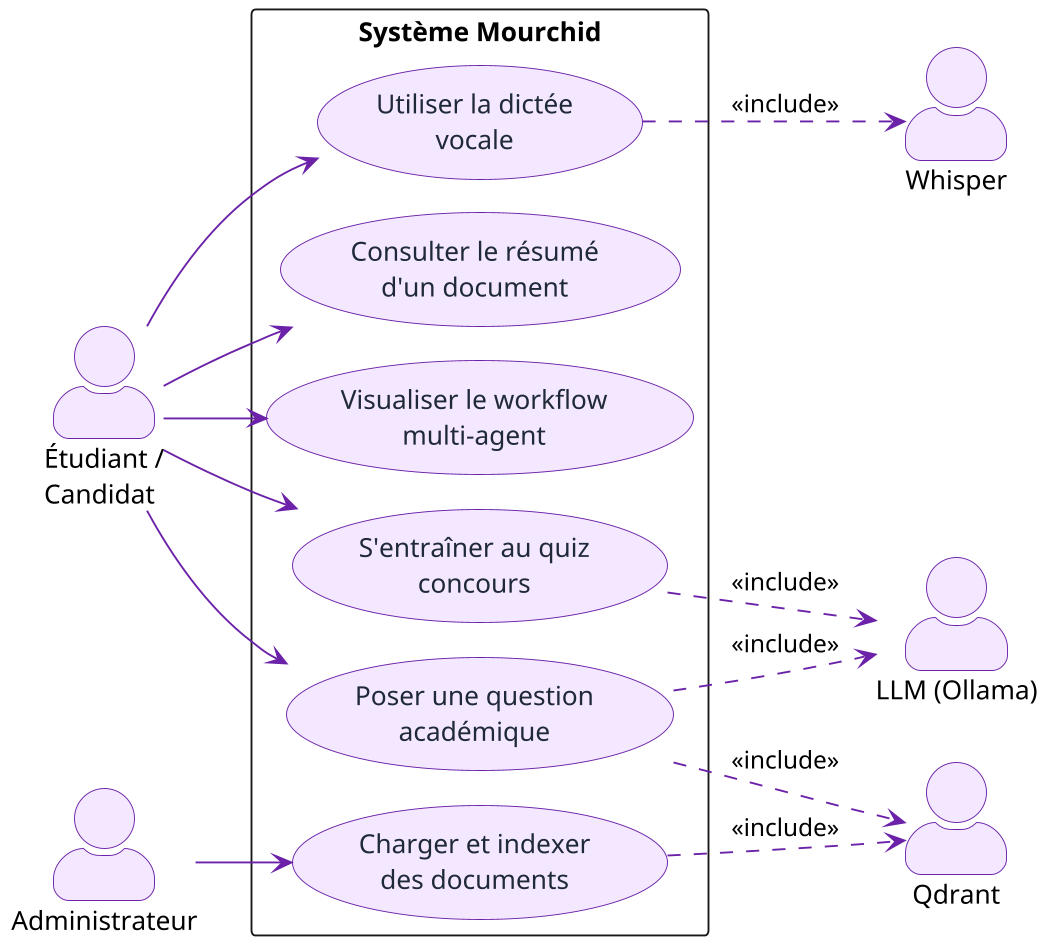
\includegraphics[width=\textwidth]{uml/use_case.png}
\caption{Diagramme de cas d'utilisation --- système Mourchid (généré avec PlantUML).}
\end{figure}

\subsection{Diagramme de classes}

\begin{figure}[H]
\centering
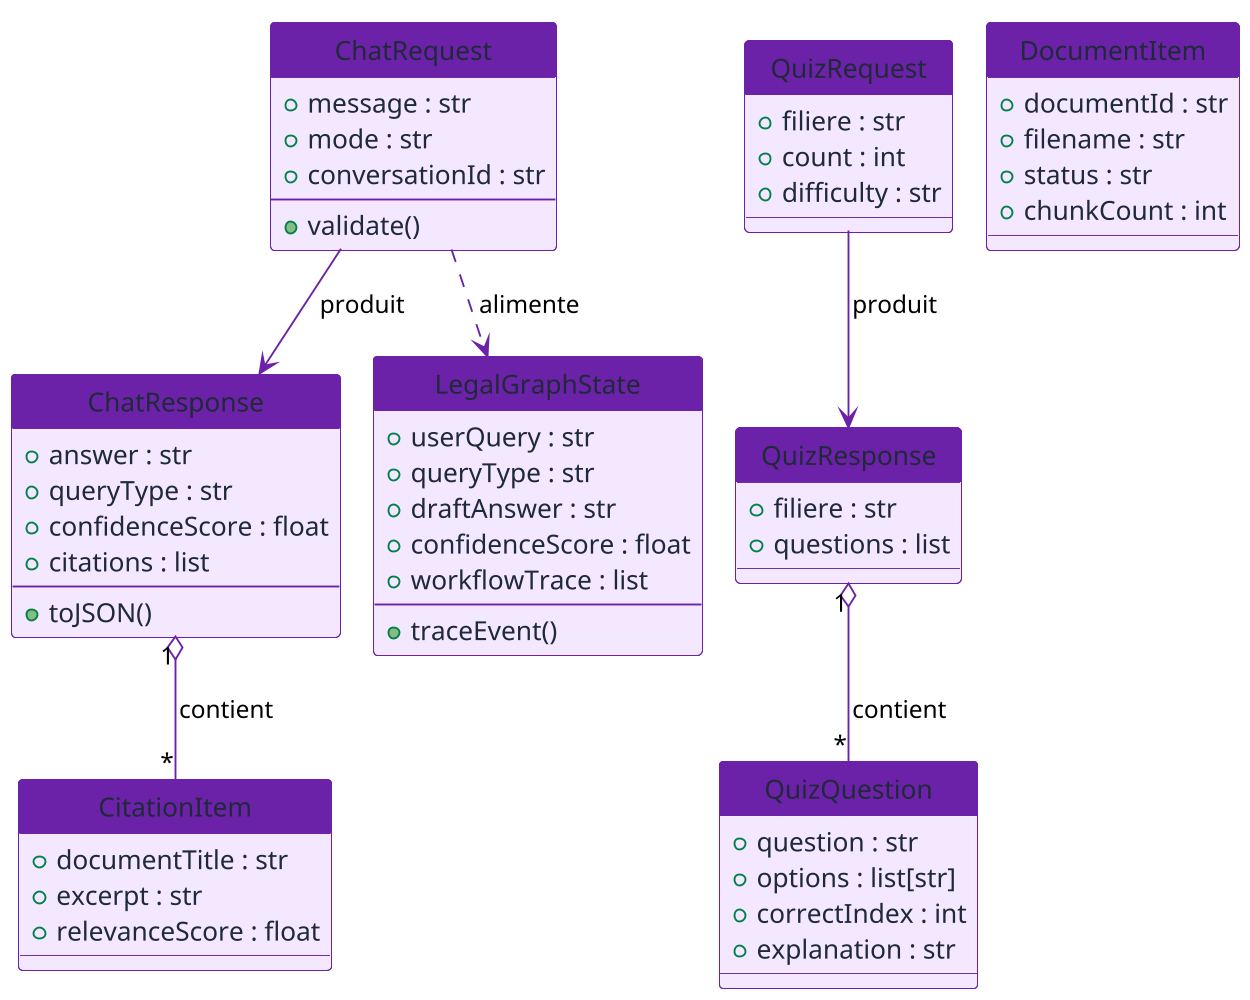
\includegraphics[width=\textwidth]{uml/class_diagram.png}
\caption{Diagramme de classes --- modèles de données de l'API Mourchid (généré avec PlantUML).}
\end{figure}

\subsection{Diagramme de séquence --- flux de chat (streaming SSE)}

\begin{figure}[H]
\centering
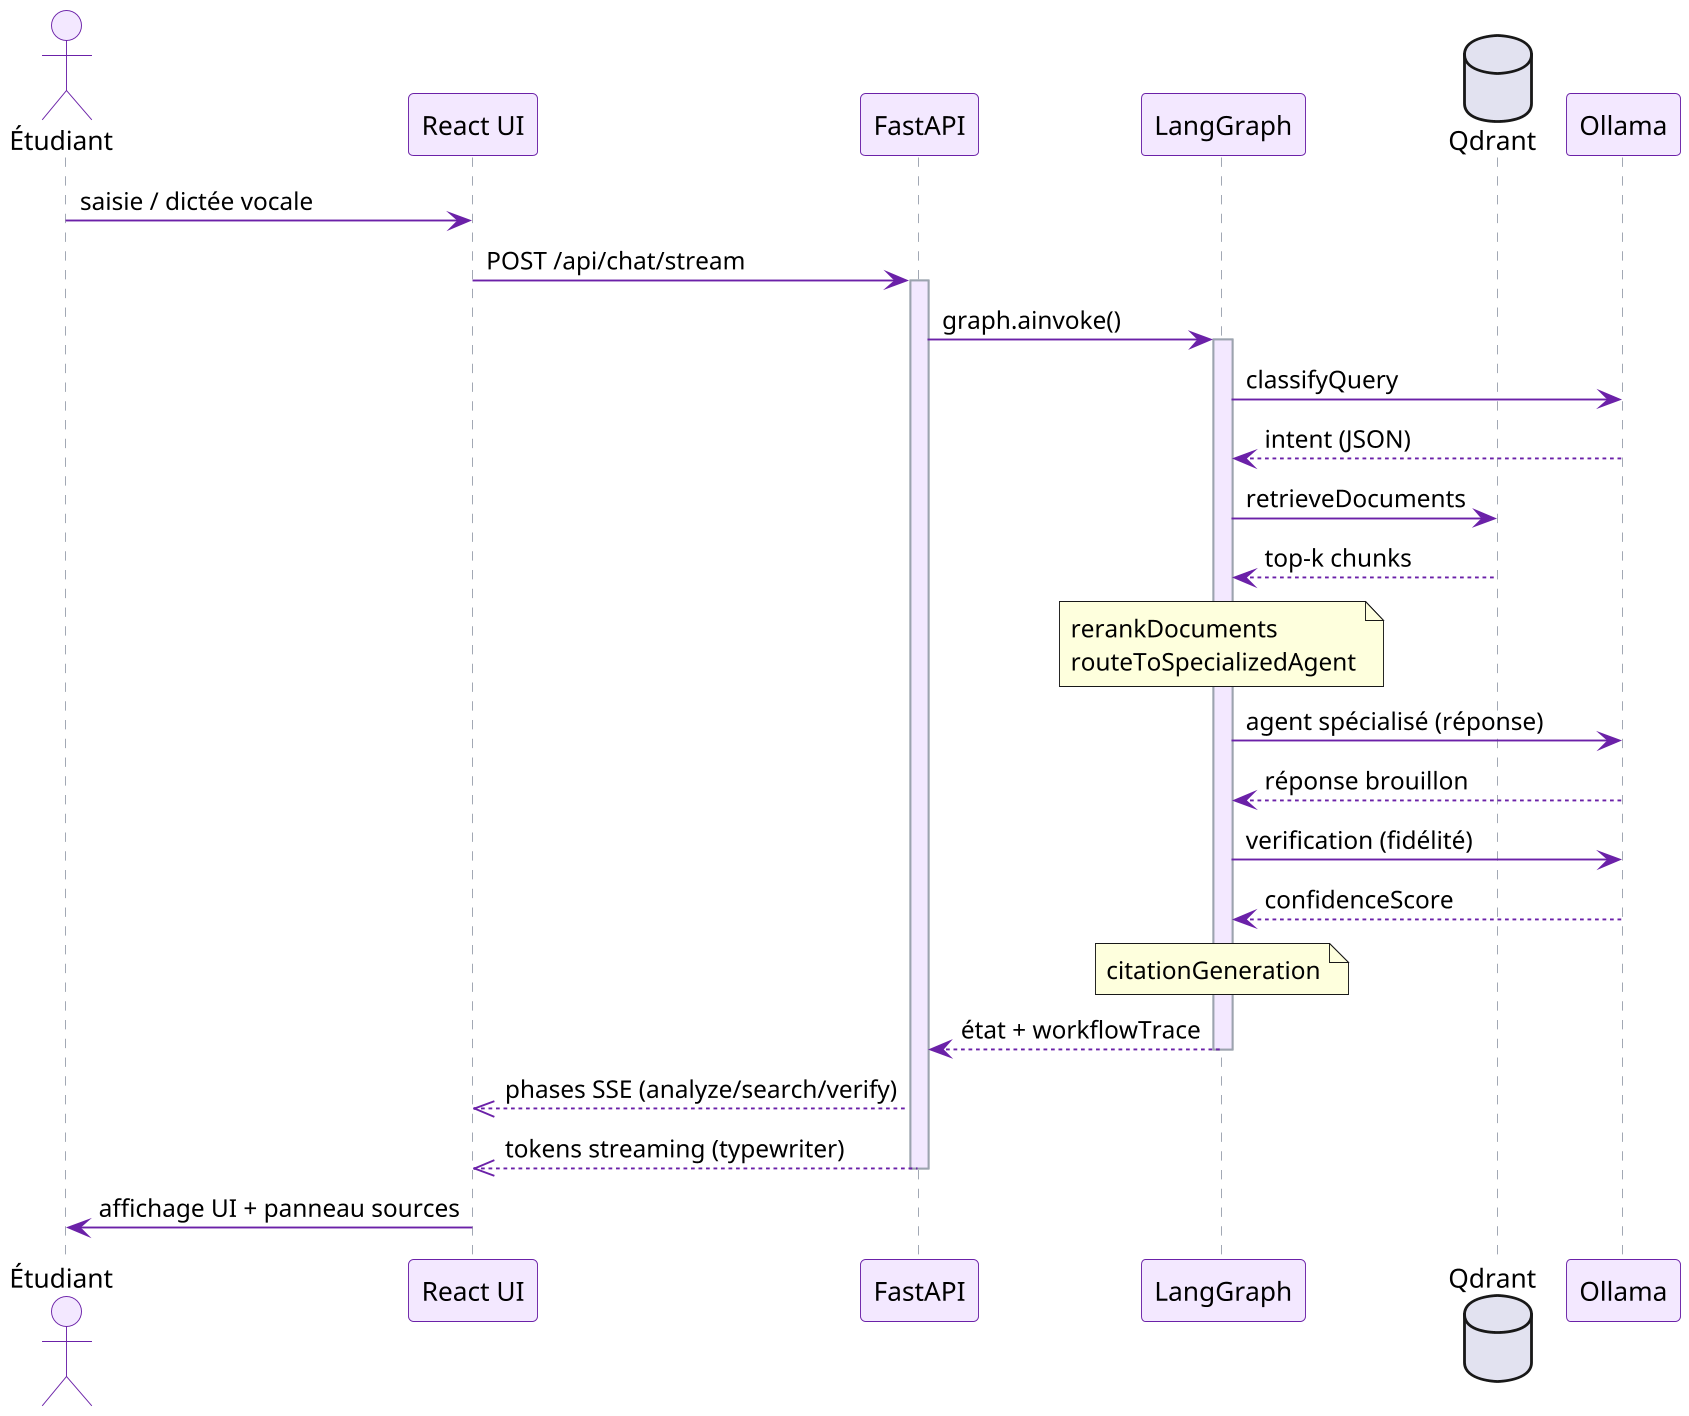
\includegraphics[width=\textwidth,height=0.82\textheight,keepaspectratio]{uml/sequence_chat.png}
\caption{Diagramme de séquence UML --- parcours chat avec streaming SSE multi-agent (généré avec PlantUML).}
\end{figure}

\subsection{Diagramme de séquence --- dictée vocale (Whisper)}

\begin{figure}[H]
\centering
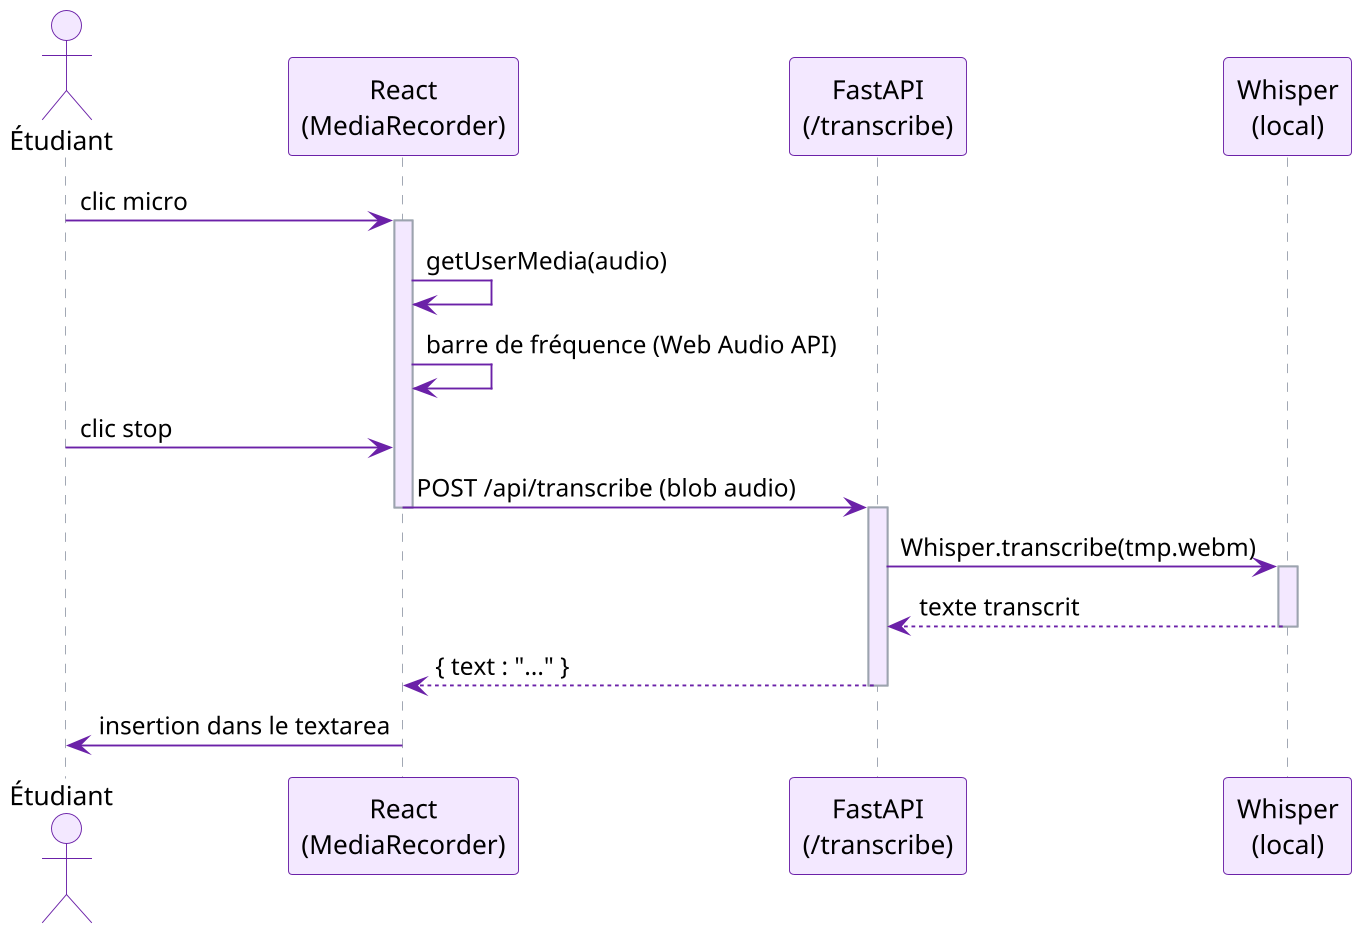
\includegraphics[width=0.85\textwidth]{uml/sequence_voice.png}
\caption{Diagramme de séquence --- dictée vocale et transcription Whisper côté serveur (généré avec PlantUML).}
\end{figure}

% =============================================================================
\section{Conception technique}

\subsection{Architecture générale}

L'application suit une architecture \textbf{monorepo} séparant clairement le backend Python et le frontend TypeScript, communiquant via \textbf{API REST} et \textbf{Server-Sent Events (SSE)}.

\begin{figure}[H]
\centering
\begin{tikzpicture}[
  node distance=1.2cm and 2cm,
  box/.style={rectangle, rounded corners=5pt, draw=mypurple, fill=mypurplelight!40,
    minimum width=2.8cm, minimum height=0.8cm, align=center, font=\sffamily\footnotesize},
  storage/.style={cylinder, shape border rotate=90, draw=mypurple!70, fill=mypurplelight!20,
    minimum width=1.8cm, minimum height=0.8cm, align=center, font=\sffamily\footnotesize},
  arr/.style={->, thick, mypurple!80}
]
\node[box] (react)  {React + Vite\\TypeScript};
\node[box, right=3cm of react] (fastapi) {FastAPI\\Python 3.11};
\node[box, right=2.5cm of fastapi] (lg) {LangGraph\\11 nœuds};
\node[box, below=1.5cm of lg] (rag) {RAG Retriever\\SentenceTransformers};
\node[storage, left=2cm of rag] (qdrant) {Qdrant};
\node[box, right=2cm of rag] (ollama) {Ollama\\LLM local};
\node[box, below=1.5cm of fastapi] (whisper) {Whisper\\(Transcription)};

\draw[arr] (react) -- node[above, font=\tiny]{REST + SSE} (fastapi);
\draw[arr] (fastapi) -- (lg);
\draw[arr] (lg) -- (rag);
\draw[arr] (rag) -- (qdrant);
\draw[arr] (lg) -- (ollama);
\draw[arr] (fastapi) -- (whisper);
\draw[arr, dashed] (lg) -- node[right, font=\tiny]{quiz / résumé} (ollama);
\end{tikzpicture}
\caption{Architecture logique du projet Mourchid.}
\end{figure}

\subsection{Stack technologique}

\begin{table}[H]
    \centering
    \sffamily\renewcommand{\arraystretch}{1.35}
    \begin{tabularx}{\textwidth}{>{\bfseries}p{2.5cm} X >{\centering\arraybackslash}p{2.5cm}}
        \toprule
        \rowcolor{mypurple}
        \textcolor{white}{Couche} & \textcolor{white}{Technologies} & \textcolor{white}{Version} \\
        \midrule
        Frontend & React, TypeScript, Vite, Tailwind CSS, Framer Motion, Radix UI & React 18 / Vite 5 \\
        \rowcolor{codegray}
        Backend API & Python, FastAPI, Uvicorn, SSE & Python 3.11+ \\
        Orchestration & LangGraph (graphe d'agents typé, traces persistées) & 0.2+ \\
        \rowcolor{codegray}
        RAG / Embeddings & SentenceTransformers (\texttt{multilingual-e5-base}), Qdrant & --- \\
        LLM & Ollama (local, \texttt{mistral}, \texttt{llama3.1}…) & --- \\
        \rowcolor{codegray}
        Transcription & Whisper via HuggingFace Transformers, PyTorch, FFmpeg & whisper-base \\
        Packaging & uv (Python), npm (Node) & --- \\
        \rowcolor{codegray}
        Déploiement & Docker Compose (Qdrant + backend + frontend) & --- \\
        \bottomrule
    \end{tabularx}
    \caption{Stack technologique open-source du projet.}
\end{table}

\subsection{Structure du dépôt}

\begin{filetree}
\ftdir{enset-assistant/}
\ftitem{backend/}{FastAPI + LangGraph + RAG + MCP (uv)}
\ftitem{\ \ app/main.py}{Point d'entrée API (routes + CORS)}
\ftitem{\ \ app/api/}{routes\_chat, routes\_quiz, routes\_transcribe, routes\_documents…}
\ftitem{\ \ app/agents/}{quiz\_agent, summary\_agent, citation\_agent, verification\_agent…}
\ftitem{\ \ app/graph/}{legal\_workflow.py (LangGraph), state.py, nodes.py, conditions.py}
\ftitem{\ \ app/rag/}{embeddings, retriever, vector\_store, chunker, indexer}
\ftitem{\ \ app/llm/}{local\_llm.py (Ollama / llama.cpp), prompts.py}
\ftitem{\ \ app/services/}{chat\_service, quiz\_service, transcription\_service, summary\_service…}
\ftitem{\ \ app/data/samples/}{Corpus académique ENSET (Markdown)}
\ftitem{\ \ pyproject.toml}{Dépendances Python (uv)}
\ftdir{frontend/}
\ftitem{src/pages/}{Chat.tsx, Quiz.tsx, Workflow.tsx, Dashboard.tsx, Summary.tsx}
\ftitem{src/components/}{chat/ (ChatComposer, VoiceVisualizer, MessageCard…), layout/ (Sidebar)}
\ftitem{src/services/api.ts}{Appels REST (streamChat, generateQuiz, transcribeAudio…)}
\ftitem{src/types/}{index.ts, speech.d.ts}
\ftdir{screens/}
\ftitem{assistant.png, transcription.png}{Captures interface chat et dictée vocale}
\ftitem{QuizCncr.png, document.png}{Captures quiz et gestion documentaire}
\ftitem{workFlow.png, dashboard.png, resumedocsEnset.png}{Autres écrans}
\ftitem{docker-compose.yml}{Stack complète (Qdrant + backend + frontend)}
\end{filetree}

\subsection{Graphe LangGraph}

Le cœur de l'application est un \textbf{graphe d'agents LangGraph} comportant \textbf{11 nœuds} interconnectés avec routage conditionnel :

\begin{figure}[H]
\centering
\begin{tikzpicture}[
  font=\sffamily\scriptsize,
  node distance=0.6cm and 1.4cm,
  n/.style={rectangle, rounded corners=3pt, draw=mypurple, fill=mypurplelight!35,
    minimum width=2.6cm, minimum height=0.6cm, align=center},
  branch/.style={rectangle, rounded corners=3pt, draw=mypurple!60, fill=mypurplelight!20,
    minimum width=2cm, minimum height=0.6cm, align=center},
  arr/.style={->, mypurple!80, thick},
  cond/.style={->, mypurple!50, dashed}
]
\node[n] (start) {START};
\node[n, below=of start] (classify) {classifyQuery};
\node[n, below=of classify] (retrieve) {retrieveDocuments};
\node[n, below=of retrieve] (rerank) {rerankDocuments};
\node[n, below=of rerank] (route) {routeToSpecializedAgent};

\node[branch, below left=0.8cm and 2.2cm of route] (acad) {academicAnswer};
\node[branch, below=0.8cm of route] (proc) {procedureAnalysis};
\node[branch, below right=0.8cm and 2.2cm of route] (summ) {summaryAnalysis};
\node[branch, right=1.4cm of summ] (comp) {comparisonAnalysis};

\node[n, below=2.4cm of route] (cit) {citationGeneration};
\node[n, below=of cit] (verif) {verification};
\node[n, below=of verif] (final) {finalResponse};
\node[n, below=of final] (end) {END};

\draw[arr] (start) -- (classify);
\draw[arr] (classify) -- node[right, font=\tiny]{continue} (retrieve);
\draw[cond] (classify.east) to[out=0, in=0] node[right, font=\tiny]{out\_of\_scope} (final.east);
\draw[arr] (retrieve) -- (rerank);
\draw[arr] (rerank) -- (route);
\draw[cond] (route) -- (acad);
\draw[cond] (route) -- (proc);
\draw[cond] (route) -- (summ);
\draw[cond] (route) -- (comp);
\draw[arr] (acad) |- (cit);
\draw[arr] (proc) -- (cit);
\draw[arr] (summ) |- (cit);
\draw[arr] (comp) |- (cit);
\draw[arr] (cit) -- (verif);
\draw[arr] (verif) -- (final);
\draw[arr] (final) -- (end);
\end{tikzpicture}
\caption{Graphe LangGraph du pipeline multi-agent Mourchid (11 nœuds).}
\end{figure}

\subsection{Endpoints REST principaux}

\begin{table}[H]
    \centering
    \sffamily\footnotesize\renewcommand{\arraystretch}{1.25}
    \begin{tabularx}{\textwidth}{l l X}
        \toprule
        \rowcolor{mypurple}
        \textcolor{white}{\textbf{Méthode}} & \textcolor{white}{\textbf{Route}} & \textcolor{white}{\textbf{Description}} \\
        POST & /api/chat & Chat RAG agentic (réponse, citations, confiance, trace) \\
        \rowcolor{codegray}
        POST & /api/chat/stream & SSE : phases multi-agent + tokens streaming \\
        POST & /api/quiz & Quiz QCM généré par le LLM (filière, difficulté) \\
        \rowcolor{codegray}
        POST & /api/transcribe & Transcription Whisper depuis un blob audio \\
        POST & /api/summarize & Résumé structuré (points clés, obligations, risques) \\
        \rowcolor{codegray}
        POST & /api/documents/upload & Upload d'un fichier dans le corpus \\
        POST & /api/documents/index & Indexation / réindexation du corpus \\
        \rowcolor{codegray}
        GET  & /api/workflow/trace/\{id\} & Trace d'exécution persistée par conversation \\
        GET  & /api/health & État LLM, base vectorielle, modèle d'embedding \\
        \bottomrule
    \end{tabularx}
    \caption{API REST FastAPI exposée au frontend React.}
\end{table}

\subsection{Composant de dictée vocale}

\begin{vscodebox}{ChatComposer.tsx — dictée vocale (MediaRecorder + Whisper)}
async function startRecording() {
  const media = await navigator.mediaDevices.getUserMedia({ audio: true });
  setStream(media);            // → VoiceVisualizer (Web Audio API)
  const recorder = new MediaRecorder(media);
  recorder.onstop = async () => {
    const blob = new Blob(chunks, { type: recorder.mimeType });
    const text = await transcribeAudio(blob); // POST /api/transcribe
    setText(prev => prev ? `${prev} ${text}` : text);
  };
  recorder.start();
}
\end{vscodebox}

\begin{vscodebox}{transcription\_service.py — pipeline Whisper côté serveur}
@lru_cache(maxsize=1)
def _get_pipeline():
    return pipeline(
        "automatic-speech-recognition",
        model=settings.whisper_model,   # openai/whisper-base par defaut
        device=0 if torch.cuda.is_available() else -1,
        chunk_length_s=30,
    )

async def transcribe_audio(content: bytes, filename: str) -> str:
    with tempfile.NamedTemporaryFile(suffix=".webm") as tmp:
        tmp.write(content)
        result = _get_pipeline()(tmp.name, generate_kwargs={
            "language": "french", "task": "transcribe"
        })
    return result["text"].strip()
\end{vscodebox}

\subsection{Génération de quiz par le LLM}

\begin{vscodebox}{quiz\_agent.py — génération de quiz via LLM}
async def generate_quiz(llm, filiere, count=5, difficulty="moyen"):
    user = (f"Filiere: {filiere}\nNombre: {count}\n"
            f"Difficulte: {difficulty}\nGenere un quiz original.")
    # temperature=0.9 pour varier le quiz a chaque appel
    raw = await llm.complete(QUIZ_SYSTEM, user, temperature=0.9, json_mode=True)
    data = safe_parse_json(raw)
    return data.get("questions", [])
\end{vscodebox}

% =============================================================================
\section{Réalisation}

\subsection{Interface assistant académique}

\screenshot{0.95}{assistant.png}{Page Assistant --- chat RAG en streaming SSE avec suggestions de questions, sélecteur de niveau (Simple / Détaillé / Technique / Procédure), questions prédéfinies et panneau latéral « Analyse \& sources » affichant les citations, les extraits RAG et le score de confiance.}

\subsection{Dictée vocale avec barre de fréquence}

\screenshot{0.95}{transcription.png}{Dictée vocale --- enregistrement audio via \texttt{MediaRecorder}, visualisation en temps réel de l'amplitude par une barre de fréquence (Web Audio API + Canvas), puis transcription automatique via Whisper côté serveur et insertion du texte dans la zone de saisie.}

\subsection{Quiz concours généré par l'IA}

\screenshot{0.95}{QuizCncr.png}{Quiz concours --- sélection de la filière (Génie Informatique, Électrique, Mécanique) et du niveau de difficulté ; chaque quiz est généré à la demande par le LLM (QCM avec 4 options, bonne réponse et explication pédagogique). L'interface affiche une barre de progression et une correction détaillée en fin de session.}

\subsection{Gestion documentaire}

\screenshot{0.95}{document.png}{Gestion du corpus documentaire --- upload de fichiers PDF, Markdown ou texte, réindexation globale, statut d'indexation par fichier (nombre de chunks, identifiant). L'indexation alimente la base vectorielle Qdrant via les SentenceTransformers.}

\subsection{Visualisation du workflow multi-agent}

\screenshot{0.95}{workFlow.png}{Page Workflow --- visualisation de la trace d'exécution du pipeline LangGraph par \texttt{conversationId} : chaque nœud (classifyQuery, retrieveDocuments, rerankDocuments, agent spécialisé, citationGeneration, verification, finalResponse) est affiché avec son détail et ses données de payload.}

\subsection{Tableau de bord}

\screenshot{0.95}{dashboard.png}{Tableau de bord --- statistiques d'utilisation (documents indexés, questions posées, taux de vérification réussi), modèles utilisés (LLM, embeddings, base vectorielle) et historique des dernières requêtes.}

\subsection{Résumé structuré de documents}

\screenshot{0.95}{resumedocsEnset.png}{Page Résumé --- saisie d'un texte académique ou collage d'un document, puis synthèse structurée générée par le LLM : résumé principal, points clés, obligations, risques et articles de référence.}

% =============================================================================
\section{Installation et déploiement}

\setcounter{stepcounter}{0}

\begin{etapebox}
\textbf{Base vectorielle Qdrant}
\begin{terminalbox}[sdia@enset:~/enset-assistant]
(*@\textcolor{ubuntugreen}{docker run -d -p 6333:6333 qdrant/qdrant}@*)
\end{terminalbox}
\end{etapebox}

\begin{etapebox}
\textbf{Backend Python} (depuis \texttt{backend/}) --- dépendances, corpus, serveur :
\begin{terminalbox}[sdia@enset:~/enset-assistant/backend]
(*@\textcolor{ubuntugreen}{uv sync --group dev}@*)
(*@\textcolor{ubuntugreen}{cp ../.env.example .env}@*)
(*@\textcolor{ubuntugreen}{uv run python -m app.scripts.seed\_index}@*)
(*@\textcolor{ubuntugreen}{uv run uvicorn app.main:app --reload --port 8000}@*)
\end{terminalbox}
\end{etapebox}

\begin{etapebox}
\textbf{LLM Ollama} (sur l'hôte) :
\begin{terminalbox}[sdia@enset:~/enset-assistant]
(*@\textcolor{ubuntugreen}{ollama serve}@*)
(*@\textcolor{ubuntugreen}{ollama pull mistral}@*)
\end{terminalbox}
\end{etapebox}

\begin{etapebox}
\textbf{Frontend React} (depuis \texttt{frontend/}) :
\begin{terminalbox}[sdia@enset:~/enset-assistant/frontend]
(*@\textcolor{ubuntugreen}{npm install}@*)
(*@\textcolor{ubuntugreen}{npm run dev}@*)
(*@\textcolor{ubuntutext}{\# Interface disponible sur http://localhost:5173}@*)
\end{terminalbox}
\end{etapebox}

\begin{alertsuccess}[Checklist de validation]
\begin{itemize}\setlength{\itemsep}{0.2em}
    \item \texttt{GET /api/health} renvoie \texttt{status: ok}
    \item L'assistant répond avec citations et score de confiance
    \item La dictée vocale transcrit correctement (Whisper se charge au 1er appel)
    \item Le quiz est différent à chaque génération pour une même filière
\end{itemize}
\end{alertsuccess}

\begin{alertwarning}[Premier lancement]
Au premier appel à la transcription vocale, le modèle Whisper (\texttt{openai/whisper-base}, \(\approx\)290 Mo) est téléchargé automatiquement depuis HuggingFace. Ce chargement initial est unique et mis en cache localement.
\end{alertwarning}

% =============================================================================
\section{Conclusion}

\subsection{Résumé du projet}

Le projet \textbf{Mourchid} démontre la faisabilité d'un assistant académique intelligent \textbf{local-first} et \textbf{open-source} répondant à un besoin réel des étudiants et candidats de l'ENSET Mohammedia. Il intègre avec succès :

\begin{itemize}
    \item Un \textbf{pipeline RAG agentique} complet (Qdrant + SentenceTransformers + LangGraph) garantissant des réponses sourcées et auditables.
    \item Un \textbf{streaming SSE multi-phase} pour une expérience utilisateur fluide et transparente.
    \item Une \textbf{dictée vocale} robuste fonctionnant sur tous les navigateurs, grâce à la transcription Whisper côté serveur.
    \item Un \textbf{quiz concours dynamique} généré par l'IA, offrant un entraînement personnalisé par filière et par difficulté.
    \item Une architecture \textbf{100\% locale} : aucune donnée n'est envoyée à des services tiers.
\end{itemize}

\subsection{Défis rencontrés}

\begin{table}[H]
    \centering
    \sffamily\footnotesize\renewcommand{\arraystretch}{1.3}
    \begin{tabularx}{\textwidth}{>{\bfseries}p{4cm} X}
        \toprule
        \rowcolor{mypurple}
        \textcolor{white}{Défi} & \textcolor{white}{Solution adoptée} \\
        \midrule
        Transcription vocale sur Linux & Abandon de l'API Web Speech (non fiable sur Chromium/Linux) au profit de Whisper côté serveur via \texttt{MediaRecorder}. \\
        \rowcolor{codegray}
        Variabilité des quiz LLM & Température élevée (0.9) pour diversifier les sorties + nettoyage robuste des questions mal formées. \\
        Streaming bloquant le thread & Utilisation d'\texttt{asyncio.create\_task} pour exécuter le graphe LangGraph en parallèle des événements SSE. \\
        \rowcolor{codegray}
        Hallucinations RAG & Nœud \texttt{verification} post-génération évaluant la fidélité aux extraits + message de repli si insuffisance documentaire. \\
        Port occupé au redémarrage & Processus root lancé par \texttt{uv run} — résolu par \texttt{sudo fuser -k 8000/tcp} puis relance avec \texttt{--reload}. \\
        \bottomrule
    \end{tabularx}
    \caption{Principaux défis et solutions apportées.}
\end{table}

\subsection{Recommandations et perspectives}

\begin{itemize}
    \item \textbf{Enrichissement du corpus} : indexer les guides officiels, règlements pédagogiques et emplois du temps réels de l'ENSET.
    \item \textbf{Support arabe} : les champs de métadonnées sont prévus ; une interface bilingue (FR/AR) est envisageable.
    \item \textbf{Human-in-the-loop renforcé} : activer le mécanisme \texttt{interrupt} de LangGraph avant \texttt{finalResponse} pour permettre à un modérateur de valider les réponses sensibles.
    \item \textbf{Whisper Large} : migrer vers \texttt{whisper-small} ou \texttt{whisper-large} pour une meilleure précision en français et en darija.
    \item \textbf{Déploiement hébergé} : conteneuriser via Docker Compose et déployer sur un serveur ENSET pour un accès centralisé sans installation locale.
    \item \textbf{Mobile-first} : adapter l'interface responsive pour une utilisation optimale sur smartphone (accès rapide à la dictée vocale en mobilité).
\end{itemize}

\begin{citationbox}
Mourchid illustre comment les technologies d'intelligence artificielle distribuée --- orchestration multi-agent (LangGraph), RAG vectoriel (Qdrant), transcription neurale locale (Whisper) et génération LLM (Ollama) --- peuvent être assemblées en une application web cohérente, ouverte et souveraine, au service de la communauté académique de l'ENSET Mohammedia.
\end{citationbox}

\end{document}
